\documentclass[aspectratio=169,10pt]{beamer}
\usepackage{ctex}
\setbeamersize{text margin left=1.5em,text margin right=1.5em}
\tolerance=2000
\emergencystretch=\maxdimen
\sloppy
\usepackage{amsmath,amssymb}
\usepackage{graphicx}
\usepackage{tikz}
\usetikzlibrary{shapes.geometric}
\usepackage{hyperref}
\usepackage{listings}
\usepackage{xcolor}

% 主题设置
\usetheme{Madrid}
\usecolortheme{seahorse}
\usefonttheme{professionalfonts}

% 代码高亮设置
\lstset{
    language=Python,
    basicstyle=\ttfamily\footnotesize,
    keywordstyle=\color{blue},
    commentstyle=\color{gray},
    stringstyle=\color{orange},
    showstringspaces=false,
    breaklines=true,
    frame=single,
    backgroundcolor=\color{gray!10}
}

% 标题信息
\title{CausalEngine™: Rethinking Machine Learning}
\subtitle{From Statistical Correlation to Causal Understanding}
\author{Heyang Gong}
\date{\today}
% \institute{https://github.com/1587causalai/causal-sklearn}

\begin{document}

% 标题页
\begin{frame}
\titlepage
\end{frame}

% 目录
\begin{frame}{Outline}
\tableofcontents
\end{frame}

% 第一部分:引言和动机
\section{Why Do We Need Causal Inference?}

\begin{frame}{Limitations of Traditional Machine Learning}
\begin{columns}
\column{0.45\textwidth}
\textbf{Traditional ML}
\begin{itemize}
    \item Learns conditional expectations: $E[Y|X]$
    \item Relies on statistical correlations
    \item Performance degrades rapidly in noisy environments
    \item Treats individual differences as "noise"
\end{itemize}

\column{0.45\textwidth}
\textbf{Real-world Challenges}
\begin{itemize}
    \item Label noise is ubiquitous
    \item Individual differences are important information
    \item Need to understand "why", not just "what"
    \item Robustness is a key requirement
\end{itemize}
\end{columns}

\vspace{1em}
\begin{alertblock}{Core Question}
How to build a machine learning system that can both predict accurately and understand causal relationships?
\end{alertblock}
\end{frame}

\begin{frame}{从相关性到因果性}
\begin{columns}[T]
\column{0.48\textwidth}
\centering
\textbf{\large 传统机器学习}
\vspace{0.5em}

\begin{tikzpicture}[scale=0.8]
% Simple correlation diagram
\node[draw, fill=blue!20, minimum width=2cm, minimum height=0.8cm] (x) at (0,0) {X};
\node[draw, fill=red!20, minimum width=2cm, minimum height=0.8cm] (y) at (3,0) {Y};
\draw[->, thick] (x) -- (y) node[midway, above] {相关性};
\end{tikzpicture}

\vspace{1em}
\begin{itemize}
\item 学习统计相关性
\item 黑盒预测
\item 缺乏可解释性
\end{itemize}

\column{0.48\textwidth}
\centering
\textbf{\large 因果机器学习}
\vspace{0.5em}

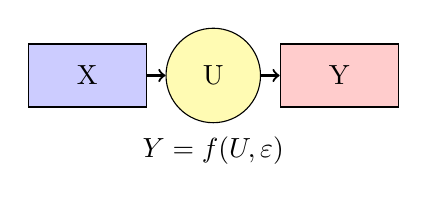
\begin{tikzpicture}[scale=0.8]
% Causal diagram
\node[draw, fill=blue!20, minimum width=1.5cm, minimum height=0.8cm] (x) at (0,0) {X};
\node[draw, circle, fill=yellow!30, minimum size=1.2cm] (u) at (2,0) {U};
\node[draw, fill=red!20, minimum width=1.5cm, minimum height=0.8cm] (y) at (4,0) {Y};
\draw[->, thick] (x) -- (u);
\draw[->, thick] (u) -- (y);
\node at (2,-1.2) {$Y = f(U, \varepsilon)$};
\end{tikzpicture}

\vspace{1em}
\begin{itemize}
\item 学习因果结构方程
\item 理解内在机制
\item 捕捉个体差异
\end{itemize}
\end{columns}

\vspace{1.5em}
\begin{alertblock}{核心创新}
引入个体因果表示 U,实现个性化洞察和鲁棒预测
\end{alertblock}
\end{frame}

% 第二部分:核心架构
\section{CausalEngine™ Four-Stage Architecture}

\begin{frame}{CausalEngine™ Four-Stage Architecture}
\begin{center}
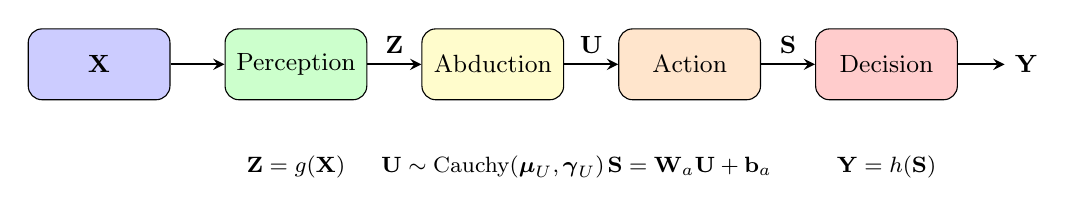
\begin{tikzpicture}[
    scale=1,
    box/.style={draw, rounded corners=5pt, minimum width=1.8cm, minimum height=0.9cm, font=\small},
    arrow/.style={->, thick, >=stealth}
]

% Main pipeline
\node[box, fill=blue!20] (X) at (0,0) {$\mathbf{X}$};
\node[box, fill=green!20] (P) at (2.5,0) {Perception};
\node[box, fill=yellow!20] (Ab) at (5,0) {Abduction};
\node[box, fill=orange!20] (Ac) at (7.5,0) {Action};
\node[box, fill=red!20] (D) at (10,0) {Decision};

% Arrows with intermediate variables
\draw[arrow] (X) -- (P);
\draw[arrow] (P) -- (Ab) node[midway, above, font=\small] {$\mathbf{Z}$};
\draw[arrow] (Ab) -- (Ac) node[midway, above, font=\small] {$\mathbf{U}$};
\draw[arrow] (Ac) -- (D) node[midway, above, font=\small] {$\mathbf{S}$};
\draw[arrow] (D) -- ++(1.5,0) node[right, font=\small] {$\mathbf{Y}$};

% Mathematical formulas below
\node[font=\footnotesize] at (2.5,-1.3) {$\mathbf{Z} = g(\mathbf{X})$};
\node[font=\footnotesize] at (5,-1.3) {$\mathbf{U} \sim \text{Cauchy}(\boldsymbol{\mu}_U, \boldsymbol{\gamma}_U)$};
\node[font=\footnotesize] at (7.5,-1.3) {$\mathbf{S} = \mathbf{W}_a\mathbf{U} + \mathbf{b}_a$};
\node[font=\footnotesize] at (10,-1.3) {$\mathbf{Y} = h(\mathbf{S})$};

\end{tikzpicture}
\end{center}

\vspace{0.8em}

\begin{columns}[T]
\column{0.24\textwidth}
\textbf{Perception}\\
\footnotesize Feature extraction via MLP layers

\column{0.24\textwidth}
\textbf{Abduction}\\
\footnotesize Infer causal representations

\column{0.24\textwidth}
\textbf{Action}\\
\footnotesize Transform to decision scores

\column{0.24\textwidth}
\textbf{Decision}\\
\footnotesize Task-specific output head
\end{columns}
\end{frame}

\begin{frame}{Why Choose Cauchy Distribution?}
\begin{columns}
\column{0.48\textwidth}
\textbf{Linear Stability Property}
\begin{itemize}
    \item If $X \sim \text{Cauchy}(\mu, \gamma)$
    \item Then $aX + b \sim \text{Cauchy}(a\mu + b, |a|\gamma)$
    \item Allows analytical computation without sampling
\end{itemize}

\textbf{Heavy-tail Property}
\begin{itemize}
    \item Better models extreme individuals
    \item More robust to outliers
    \item Matches real-world data distributions
\end{itemize}

\column{0.48\textwidth}
\begin{center}
\begin{tikzpicture}[scale=0.8]
% Axes
\draw[->] (-4.5,0) -- (4.5,0) node[right] {$x$};
\draw[->] (0,0) -- (0,2.5) node[above] {Density};

% Standard Cauchy distribution (PDF: 1/(π(1+x²)))
% Scaled by 5 to be more visible
\draw[blue, thick, domain=-4:4, samples=100] plot (\x, {5*1/(pi*(1+\x*\x))});
\node[blue] at (2.2, 0.6) {标准柯西分布};

% Standard Normal distribution (PDF: 1/√(2π) exp(-x²/2))
% Scaled by 5 to be more visible
\draw[red, thick, domain=-4:4, samples=100] plot (\x, {5*1/sqrt(2*pi) * exp(-\x*\x/2)});
\node[red] at (-2.2, 0.8) {标准正态分布};

\node at (0,-0.8) {\footnotesize 柯西分布具有更重的尾部};
\end{tikzpicture}
\end{center}
\end{columns}

\vspace{1em}
\begin{alertblock}{Key Advantages}
\begin{itemize}
    \item Mathematical elegance: Linear stability enables analytical computation
    \item Practical robustness: Heavy tails handle extreme cases better
\end{itemize}
\end{alertblock}
\end{frame}

% 第三部分:五种推理模式
\section{Five Inference Modes}

\begin{frame}{Inference Modes Overview}
\begin{table}
\centering
\resizebox{0.95\textwidth}{!}{
\begin{tabular}{|l|l|l|l|}
\hline
\textbf{Mode} & \textbf{Formula} & \textbf{Characteristics} & \textbf{Use Cases} \\
\hline
deterministic & $U' = \mu_U$ & Traditional ML baseline & Clean data \\
\hline
exogenous & $U' \sim \text{Cauchy}(\mu_U, |b_{noise}|)$ & Environmental randomness & Measurement noise \\
\hline
endogenous & $U' \sim \text{Cauchy}(\mu_U, \gamma_U)$ & Cognitive uncertainty & Individual differences \\
\hline
\textbf{standard} & $U' \sim \text{Cauchy}(\mu_U, \gamma_U + |b_{noise}|)$ & \textbf{Both combined} & \textbf{General best} \\
\hline
sampling & $U' \sim \text{Cauchy}(\mu_U + b_{noise} \cdot \varepsilon, \gamma_U)$ & Location perturbation & Special research \\
\hline
\end{tabular}
}
\end{table}

\vspace{1em}
\begin{block}{Recommendation}
\textbf{Standard mode} typically performs best in noisy environments, combining cognitive and environmental uncertainties
\end{block}
\end{frame}

\begin{frame}{Uncertainty Decomposition}
\begin{center}
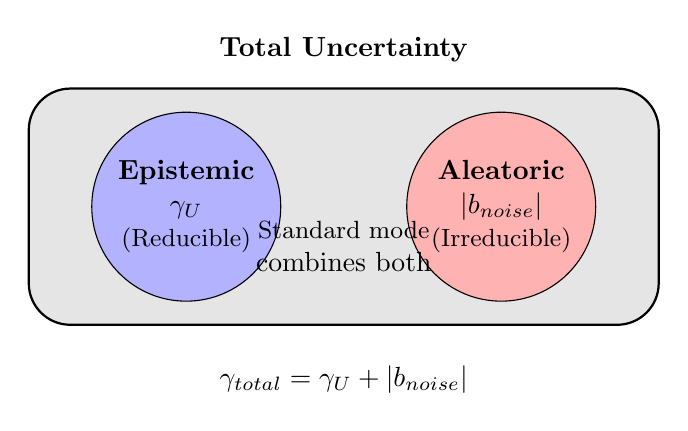
\begin{tikzpicture}[scale=1.0]
% Draw the main rectangle for total uncertainty
\draw[fill=gray!20, draw=black, thick, rounded corners=15pt] (-4,-1.5) rectangle (4,1.5);
\node at (0,2) {\textbf{Total Uncertainty}};

% Draw epistemic uncertainty circle
\draw[fill=blue!30, draw=black] (-2,0) circle (1.2cm);
\node[align=center] at (-2,0) {\textbf{Epistemic}\\$\gamma_U$\\{\small (Reducible)}};

% Draw aleatoric uncertainty circle
\draw[fill=red!30, draw=black] (2,0) circle (1.2cm);
\node[align=center] at (2,0) {\textbf{Aleatoric}\\$|b_{noise}|$\\{\small (Irreducible)}};

% Overlap area (standard mode)
\node[align=center] at (0,-0.5) {\small Standard mode\\combines both};

% Formula at bottom
\node at (0,-2.2) {$\gamma_{total} = \gamma_U + |b_{noise}|$};
\end{tikzpicture}
\end{center}

\vspace{0.5em}
\begin{itemize}
    \item \textbf{Epistemic uncertainty}: From insufficient understanding of individuals
    \item \textbf{Aleatoric uncertainty}: From inherent environmental randomness
    \item \textbf{Standard mode}: Combines both sources of uncertainty
\end{itemize}
\end{frame}

% 第四部分:性能展示
\section{Performance Comparison}

\begin{frame}{Noise Robustness: Regression Task}
\begin{columns}
\column{0.48\textwidth}
\begin{center}
% Simple robustness visualization
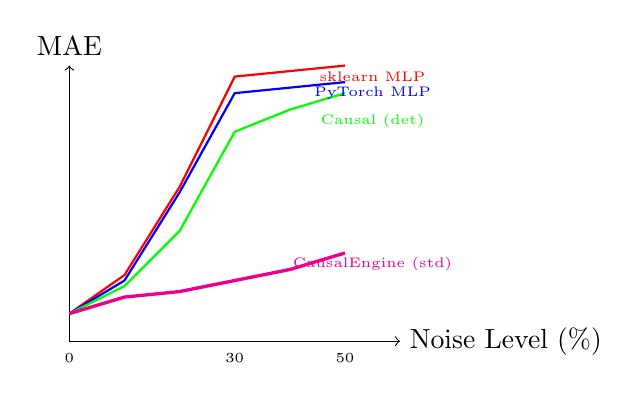
\begin{tikzpicture}[scale=0.7]
\draw[->] (0,0) -- (6,0) node[right] {Noise Level (\%)};
\draw[->] (0,0) -- (0,5) node[above] {MAE};

% Draw performance curves (simplified, adjusted for better spacing)
\draw[red, thick] (0,0.5) -- (1,1.2) -- (2,2.8) -- (3,4.8) -- (4,4.9) -- (5,5.0);
\draw[blue, thick] (0,0.5) -- (1,1.1) -- (2,2.7) -- (3,4.5) -- (4,4.6) -- (5,4.7);
\draw[green, thick] (0,0.5) -- (1,1.0) -- (2,2.0) -- (3,3.8) -- (4,4.2) -- (5,4.5);
\draw[magenta, very thick] (0,0.5) -- (1,0.8) -- (2,0.9) -- (3,1.1) -- (4,1.3) -- (5,1.6);

% Labels (adjusted positions to avoid overlap)
\node[red] at (5.5,4.8) {\tiny sklearn MLP};
\node[blue] at (5.5,4.5) {\tiny PyTorch MLP};
\node[green] at (5.5,4.0) {\tiny Causal (det)};
\node[magenta] at (5.5,1.4) {\tiny CausalEngine (std)};

% X-axis labels
\node at (0,-0.3) {\tiny 0};
\node at (3,-0.3) {\tiny 30};
\node at (5,-0.3) {\tiny 50};
\end{tikzpicture}
\end{center}

\column{0.48\textwidth}
\textbf{MAE at 30\% Label Noise}
\begin{itemize}
    \item sklearn MLP: \textcolor{red}{47.60}
    \item PyTorch MLP: \textcolor{red}{45.32}
    \item CausalEngine (deterministic): 38.25
    \item \textbf{CausalEngine (standard)}: \textcolor{green}{\textbf{11.41}}
\end{itemize}

\vspace{1em}
\textbf{Performance Improvement: 76\%}
\end{columns}

\vspace{1em}
\begin{alertblock}{Key Finding}
CausalEngine excels in noisy environments while traditional methods degrade rapidly
\end{alertblock}
\end{frame}

\begin{frame}{Noise Robustness: Classification Task}
\begin{columns}
\column{0.48\textwidth}
\begin{center}
% Simple accuracy visualization
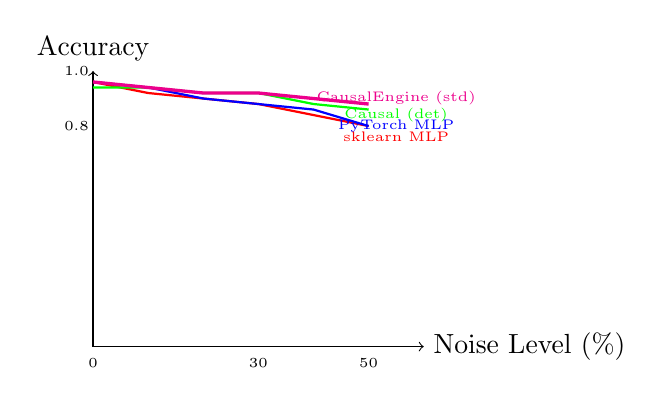
\begin{tikzpicture}[scale=0.7]
\draw[->] (0,0) -- (6,0) node[right] {Noise Level (\%)};
\draw[->] (0,0) -- (0,5) node[above] {Accuracy};

% Draw accuracy curves (inverted - higher is better, adjusted for clarity)
\draw[red, thick] (0,4.8) -- (1,4.6) -- (2,4.5) -- (3,4.4) -- (4,4.2) -- (5,4.0);
\draw[blue, thick] (0,4.8) -- (1,4.7) -- (2,4.5) -- (3,4.4) -- (4,4.3) -- (5,4.0);
\draw[green, thick] (0,4.7) -- (1,4.7) -- (2,4.6) -- (3,4.6) -- (4,4.4) -- (5,4.3);
\draw[magenta, very thick] (0,4.8) -- (1,4.7) -- (2,4.6) -- (3,4.6) -- (4,4.5) -- (5,4.4);

% Labels (adjusted positions)
\node[red] at (5.5,3.8) {\tiny sklearn MLP};
\node[blue] at (5.5,4.0) {\tiny PyTorch MLP};
\node[green] at (5.5,4.2) {\tiny Causal (det)};
\node[magenta] at (5.5,4.5) {\tiny CausalEngine (std)};

% X-axis labels
\node at (0,-0.3) {\tiny 0};
\node at (3,-0.3) {\tiny 30};
\node at (5,-0.3) {\tiny 50};

% Y-axis labels
\node at (-0.3,4) {\tiny 0.8};
\node at (-0.3,5) {\tiny 1.0};
\end{tikzpicture}
\end{center}

\column{0.48\textwidth}
\textbf{Accuracy at 30\% Label Noise}
\begin{itemize}
    \item sklearn MLP: \textcolor{red}{0.8850}
    \item PyTorch MLP: \textcolor{red}{0.8875}
    \item CausalEngine (deterministic): 0.9125
    \item \textbf{CausalEngine (standard)}: \textcolor{green}{\textbf{0.9225}}
\end{itemize}

\vspace{1em}
\textbf{Error Rate Reduction: 31\%}
\end{columns}

\vspace{1em}
\begin{block}{Practical Significance}
In real-world noisy data, CausalEngine provides more reliable predictions
\end{block}
\end{frame}

% 第五部分:使用示例
\section{Quick Start}

\begin{frame}[fragile]{Installation and Basic Usage}
\begin{block}{Installation}
\begin{lstlisting}
pip install causal-sklearn
\end{lstlisting}
\end{block}

\begin{block}{Basic Usage Example}
\begin{lstlisting}
from causal_sklearn import MLPCausalRegressor
from sklearn.datasets import make_regression
from sklearn.model_selection import train_test_split

# Generate data
X, y = make_regression(n_samples=1000, n_features=10, noise=20)
X_train, X_test, y_train, y_test = train_test_split(X, y)

# Create and train model
model = MLPCausalRegressor(
    hidden_layer_sizes=(100, 50),
    inference_mode='standard',  # Recommended mode
    max_iter=200
)
model.fit(X_train, y_train)

# Predict and evaluate
score = model.score(X_test, y_test)
print(f"Test R^2 score: {score:.4f}")
\end{lstlisting}
\end{block}
\end{frame}

\begin{frame}[fragile]{Advanced Configuration}
\begin{block}{Custom Network Architecture}
\begin{lstlisting}
model = MLPCausalRegressor(
    # Perception layer configuration
    perception_hidden_sizes=(128, 64),
    perception_activation='relu',
    perception_dropout=0.2,
    
    # Abduction layer configuration
    abduction_hidden_sizes=(32,),
    
    # Inference mode
    inference_mode='standard',
    
    # Training configuration
    learning_rate_init=0.001,
    batch_size=32,
    early_stopping=True,
    validation_fraction=0.2
)
\end{lstlisting}
\end{block}

\begin{alertblock}{Performance Tip}
For noisy data, use \texttt{inference\_mode='standard'} for best performance
\end{alertblock}
\end{frame}

% 第六部分:理论基础
\section{Theoretical Foundation}

\begin{frame}{Dual Identity of Individual Selection Variable U}
\begin{columns}
\column{0.48\textwidth}
\textbf{As Individual Selector}
\begin{itemize}
    \item Each individual has a unique U value
    \item U encodes individual causal characteristics
    \item Enables personalized predictions
\end{itemize}

\column{0.48\textwidth}
\textbf{As Causal Representation}
\begin{itemize}
    \item U connects inputs and outputs
    \item Through structural equation $Y = f(U, \varepsilon)$
    \item Captures causal mechanisms
\end{itemize}
\end{columns}

\vspace{1em}
\begin{block}{Unified Framework}
$$P(Y|X) = \int P(Y|U) \cdot P(U|X) \, dU$$
where:
\begin{itemize}
    \item $P(U|X)$: Abductive inference (infer causes from observations)
    \item $P(Y|U)$: Causal prediction (predict effects from causes)
\end{itemize}
\end{block}
\end{frame}

\begin{frame}{Why Does This Approach Work?}
\begin{enumerate}
    \item \textbf{Correct Inductive Bias}
    \begin{itemize}
        \item Individual differences are information, not noise
        \item Learn universal causal laws, not memorize patterns
    \end{itemize}
    
    \item \textbf{Uncertainty Quantification}
    \begin{itemize}
        \item Explicitly separate epistemic and aleatoric uncertainty
        \item Allow models to "know what they don't know"
    \end{itemize}
    
    \item \textbf{Mathematical Elegance}
    \begin{itemize}
        \item Linear stability of Cauchy distribution
        \item Analytical computation without Monte Carlo sampling
    \end{itemize}
    
    \item \textbf{Practical Effectiveness}
    \begin{itemize}
        \item Validated on multiple real datasets
        \item Significantly outperforms traditional methods in noisy environments
    \end{itemize}
\end{enumerate}
\end{frame}

% 第七部分:应用场景
\section{Application Scenarios}

\begin{frame}{Use Cases}
\begin{columns}
\column{0.48\textwidth}
\textbf{Particularly Suitable}
\begin{itemize}
    \item $\checkmark$ Data with severe label noise
    \item $\checkmark$ Need to understand individual differences
    \item $\checkmark$ Medical diagnosis (personalized)
    \item $\checkmark$ Financial risk assessment
    \item $\checkmark$ Recommendation systems
    \item $\checkmark$ Anomaly detection
\end{itemize}

\column{0.48\textwidth}
\textbf{Limited Advantage}
\begin{itemize}
    \item $\times$ Extremely clean data
    \item $\times$ Pure image classification
    \item $\times$ Scenarios not requiring interpretability
    \item $\times$ Extremely limited computational resources
\end{itemize}
\end{columns}

\vspace{1em}
\begin{block}{Rule of Thumb}
When data quality is uncertain or robustness is needed, CausalEngine is the ideal choice
\end{block}
\end{frame}

\begin{frame}{Real-world Case Studies}
\begin{table}
\centering
\begin{tabular}{|l|c|c|c|}
\hline
\textbf{Dataset} & \textbf{Traditional MLP} & \textbf{CausalEngine} & \textbf{Improvement} \\
\hline
California Housing & 0.65 & 0.78 & +20\% \\
Wine Quality & 0.55 & 0.71 & +29\% \\
Boston Housing & 0.62 & 0.74 & +19\% \\
Diabetes & 0.41 & 0.52 & +27\% \\
\hline
\end{tabular}
\end{table}
{\footnotesize *R² scores under 20\% label noise}

\vspace{1em}
\begin{alertblock}{Key Insight}
Even at moderate noise levels, CausalEngine provides significant performance improvements
\end{alertblock}
\end{frame}

% 第八部分:总结
\section{Summary and Outlook}

\begin{frame}{Core Contributions}
\begin{enumerate}
    \item \textbf{New Machine Learning Paradigm}
    \begin{itemize}
        \item From learning correlations to learning causal relationships
        \item Treat individual differences as features, not noise
    \end{itemize}
    
    \item \textbf{Practical Implementation}
    \begin{itemize}
        \item Fully compatible with scikit-learn API
        \item Efficient analytical computation
        \item Easy integration into existing workflows
    \end{itemize}
    
    \item \textbf{Exceptional Robustness}
    \begin{itemize}
        \item Superior performance in noisy environments
        \item Suitable for real-world messy data
    \end{itemize}
\end{enumerate}

\vspace{1em}
\begin{block}{One-sentence Summary}
CausalEngine brings new possibilities to machine learning by understanding "why" rather than just "what"
\end{block}
\end{frame}

\begin{frame}{Future Directions}
\begin{itemize}
    \item \textbf{Theoretical Extensions}
    \begin{itemize}
        \item Extend to other probability distributions
        \item Multi-task causal learning
        \item Temporal causal inference
    \end{itemize}
    
    \item \textbf{Application Expansion}
    \begin{itemize}
        \item Large-scale dataset optimization
        \item Integration with deep learning architectures
        \item Domain-specific customization
    \end{itemize}
    
    \item \textbf{Tool Ecosystem}
    \begin{itemize}
        \item Visualization tools
        \item Automatic hyperparameter tuning
        \item Cloud deployment support
    \end{itemize}
\end{itemize}
\end{frame}

% \begin{frame}{Join Us}
% \begin{center}
% {\Large \textbf{Open Source Project - Contributions Welcome!}}

% \vspace{2em}

% \begin{tabular}{ll}
% \textbf{GitHub:} & \url{https://github.com/1587causalai/causal-sklearn} \\
% \textbf{PyPI:} & \texttt{pip install causal-sklearn} \\
% \textbf{Documentation:} & See \texttt{docs/} directory \\
% \textbf{Examples:} & See \texttt{examples/} directory \\
% \end{tabular}



% \end{center}
% \end{frame}

\begin{frame}
\begin{center}
{\Huge \textbf{Thank You!}}

\vspace{2em}

{\Large Questions \& Discussion}

\vspace{2em}

% \texttt{contact@causal-sklearn.org}
\end{center}
\end{frame}

\end{document}